\documentclass{icga}
\newif\iflong\longtrue  %toggle longtrue longfalse
% if there is a shorter version, it will have less material
% \iflong
% ... long version material ...
% \fi

\usepackage{hyperref,url}
\usepackage{graphicx}
\def\Eo{\mbox{\sc Ezo}}
\def\Ec{\mbox{\sc Ezo-CNN}}
\def\Hite{\mbox{\sc Hexcited}}
\def\Hent{\mbox{\sc Hexcellent}}
\def\Mx{\mbox{\sc MoHex}}
\def\Mc{\mbox{\sc MoHex-CNN}}
\def\Sol{\mbox{\sc Solver}}
\def\Fuego{\mbox{\sc Fuego}}

\title{\sc Hex 2017: \Mx\ wins the 11$\times$11 and 13$\times$13 tournaments}
\runningtitle{ICGA}
\author{Ryan Hayward\thanks{Department of Computing Science, 
University of Alberta, Canada. Email:hayward@ualberta.ca},
Noah Weninger \thanks{CS, UAlberta, Email:nweninge@ualberta.ca}
}
\affiliation{Edmonton, Canada}
\issue{to appear in ICGA Journal}

\setcounter{page}{999}
\begin{document}
\maketitle

%\iflong
%In the longer version of the report, we include all games.
%\fi

\vspace*{-2.25in}
{\it to appear, ICGA Journal}
\vspace*{2.0in}

\begin{figure}[hbt]
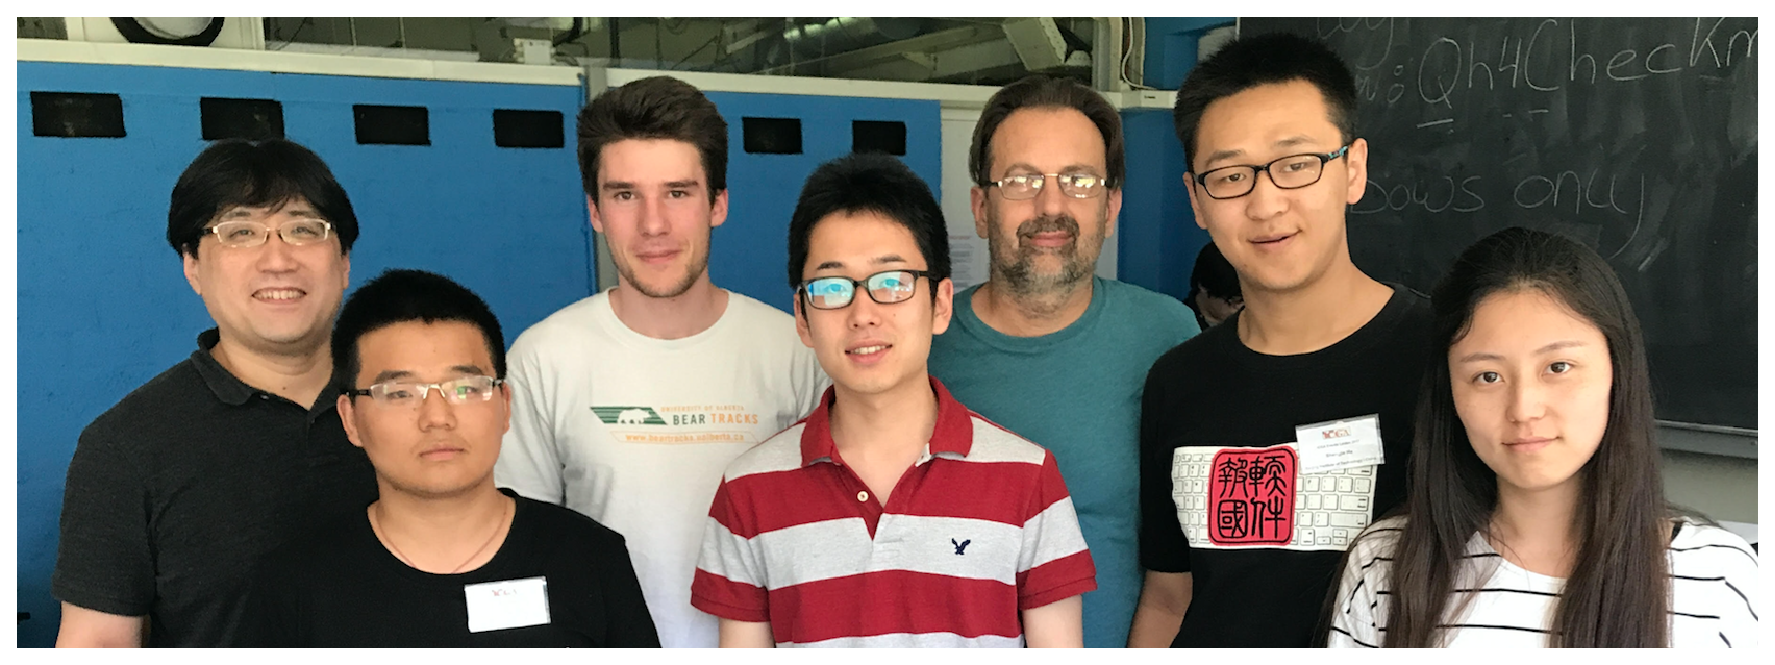
\includegraphics[width=\columnwidth]{photos/people-1.eps}\
\caption{Participants at the Hex competitions. From left,
Masahito Yamamoto,
You RunZe,
Noah Weninger,
Kei Takada,
Ryan Hayward,
Ma Shengjie,
Wu Tong.} \end{figure}

\section{The Tournaments}
There were two Hex tournaments at the 2017 Olympiad:
board size 11$\times$11 and board size 13$\times$13.
Three programs competed in each tournament.
These are at present the only annual computer Hex tournaments.
11$\times$11 is the original board size introduced by Piet Hein in 1942. 
Recently, all 1-move openings on 9$\times$9 Hex have been solved by
computers, as have two 10$\times$10 openings \citebay{PawlH13}.
So, in recent years the 13$\times$13 competition,
a preferred size in the Little Golem online Hex community \citebay{LittleG}, 
was introduced.

The 11$\times$11 contestants were
\Hite{} by Ma Shengjie from China;
\Ec{} by Kei Takada, supervised by Masahito Yamamoto, from Japan;
and \Mx{}
by Broderick Arneson, Ryan Hayward, Philip Henderson, Aja Huang, 
Jakub Pawlewicz, Noah Weninger, and Kenny Young from Canada.
The 13$\times$13 contestants were
\Hent{} by Wu Tong, operatored by You RunZe and (another, no relation)
Wu Tong from China;
\Ec{}; and
\Mc{} by Chao Gao and the \Mx\ authors from Canada.

\Mx{} \citebay{HAHMP13},
the winner of the previous seven Olympiad Hex competitions \citebay{HAHP13},
is an MCTS program that uses the Benzene Hex framework
built on the code base of \Fuego\ \citebay{fuego}.
%the Go program developed by Martin M\"{u}ller, Markus Enzenberger
%and others at the University of Alberta.
%Benzene allows virtual connection and
%inferior cell computations.
\Mx{} performs knowledge computation 
in UCT tree nodes visited at least 256 times.
\Mx{} ran on Firecreek, a 24 core shared-memory machine, 
with 4 cores reserved for the 
DFPNS solver \citebay{PawlH13}, which
produces perfect play if it solves the
position within the time allotted.
\Mx{} uses a book built by Broderick Arneson with Thomas Lincke's method 
\citebay{DBLP:conf/cg/Lincke00}. 
Noah Weninger expanded the book and added a feature
allowing the use of rotational symmetry for openings
whose rotation is in the book.
For each board size, the book covers at least eight openings.

\Mc{} is a convolutional neural net (CNN) version of \Mx{}. 
At each new node of the Monte Carlo search tree, 
a policy CNN biases child selection by
initializing child visit and win counts with artificial values.
\Mc{} ran remotely on a machine with 2 CPUs and 1 GPU.

\Ec{} is a CNN version of \Eo{}, which competed
in the 2016 and previous Olympiads.
\Eo{}, based on the Benzene framework, 
uses iterative deepening alpha-beta search 
with an evaluation function using a linear combination of
two network connectivity measures \citebay{TakadaHIY15}.
\Ec{} uses a convolutional neural policy network
for move ordering.
\Ec{} ran remotely on a machine
with two CPUs and one GPU,
with one CPU-thread for search and one CPU-thread for
Benzene's Depth-First Proof Number Search endgame solver.

\Hite{} and \Hent{} are new MCTS programs written 
respectively by Ma Shengjie and Wu Tong
of the Beijing Institute of Technology.
Each ran locally on a laptop.

Each tournament was scheduled for 8 games between
each two of the three competitors, with 30 minutes per player per game.
The tournaments started on July 1 and finished on July 5.
In most games, the losing operator resigned
soon after Benzene solved the game.
For example, in Figure~\ref{fig:EM1-3} we see that
\Ec\ resigned after \Mc\ played move 22. Can you see how black wins from here?
We give a typical playout of this game in Figure~\ref{fig:sol}.

{\large\bf 11$\times$11 Tournament.}\footnote{\citebay{H17olyrptsource}
  gives .sgf game records and other source files for this report.
  \citebay{Hexgui} gives an .sgf viewer. Smart Game Format (sgf)
  was develop by \citebay{SGF}.}
The new program \Hite{} opened strongly in several games.
For example, in its first game against \Mx, \Hite\ is in a strong
position after 15 moves, but misses the promising 16.W[g3].

Due to the late arrival of \Hite,
\Mx\ and \Ec\ played their games first.
\Ec\ and \Mx\ both use Benzene's virtual connection engine,
which give strong end games, and \Hite{} was unable to win against them.
For this reason, once the final ranking was decided,
\Hite's operator resigned its remaining games without play.

The contest for gold required a four-game playoff between \Mx{} and \Ec{},
which was not decided until the final game.

\begin{center}
{\bf
Table 1 \\
The results of the 11$\times$11 tournament
}

\begin{tabular}{|c|c|c|c|c|c|c|}
\hline {\bf id} & {\bf 11x11} &\Mx{} &\Ec{}  & \Hite{}  
                & {\bf Total} & {\bf Result} \\ 
\hline {\bf M} & \Mx{}         &      &  7-5  &  4-0   & 11-5  &  Gold \\
\hline {\bf M} & \Ec{}         &  5-7 &       &  3-0   & 8-7   &  Silver \\
\hline {\bf M} & \Hite{}       &  0-4 &  0-3  &        & 0-7   &  Bronze \\
\hline
\end{tabular}
\end{center}

\iflong
%This is the longer version, so we include all games.
%11x11 EM games
 %1 em 01 a4 s B
 %2 me 10 g2 s W
 %3 em 10 h2   B  1st win by Ezo
 %4 me 10 a2 s W
 %5 me 01 a6   W
 %6 em 10 k7 s W
 %7 me 01 a2   W
 %8 em 01 k5 s B
 %9 em 01 k6 s B
%10 me 01 a8   W

%{\bf Game 1.} {\sc E-M 0-1.} 1.B[a4] 2.W[swap] \ldots ~ ~ B wins.
%{\bf Game 2.} {\sc M-E 1-0.} 1.B[g2] 2.W[swap] \ldots ~ ~ W wins.
%{\bf Game 3.} {\sc E-M 1-0.} 1.B[h2] no swap \ldots ~ ~ B wins.
%{\bf Game 4.} {\sc M-E 0-1.} 1.B[a2] 2.W[swap] \ldots ~ ~  W wins.
%{\bf Game 5.} {\sc M-E 0-1.} 1.B[a6] no swap \ldots ~ ~  W wins.
%{\bf Game 6.} {\sc E-M 1-0.} 1.B[k7] 2.W[swap] \ldots ~ ~ W wins.
%{\bf Game 7.} {\sc M-E 0-1.} 1.B[a2] no swap \ldots ~ ~  W wins.
%{\bf Game 8.} {\sc E-M 0-1.} 1.B[k5] 2.W[swap] \ldots ~ ~ B wins.
%{\bf Playoff Game 1.} {\sc E-M 0-1.} 1.B[k6] 2.W[swap] \ldots ~ ~  B wins.
%{\bf Playoff Game 2.} {\sc M-E 0-1.} 1.B[a8] no swap \ldots ~ ~  B wins.
%{\bf Playoff Game 3.} {\sc M-E 1-0.} 1.B[a9] no swap \ldots ~ ~  B wins.
%{\bf Playoff Game 4.} {\sc E-M 0-1.} 1.B[h2] no swap \ldots ~ ~  W wins.

\begin{figure}[hbp]
\includegraphics[scale=.8]{pix/11.mh1.eps}\hspace*{-1.5cm}\
\includegraphics[scale=.8]{pix/11.hm2.eps}\hspace*{-1.5cm}\
\includegraphics[scale=.8]{pix/11.mh3.eps}\hspace*{-1.5cm}\
\includegraphics[scale=.8]{pix/11.hm4.eps}\hspace*{-1.5cm}\
\caption{\Hite-\Mx\ Games 1-4. ~ ~ M-H 1-0 ~ ~ H-M 0-1 ~ ~ M-H 1-0 ~ ~ H-M 0-1}
\end{figure}

\begin{figure}[hbp]
\includegraphics[scale=1]{pix/11.eh1.eps}\hspace*{-1.2cm}\
\includegraphics[scale=1]{pix/11.he2.eps}\hspace*{-1.2cm}\
\includegraphics[scale=1]{pix/11.eh3.eps}\hspace*{-1.2cm}\
\caption{\Hite-\Ec\ Games 1-3. ~ ~ E-H 1-0 ~ ~ H-E 0-1 ~ ~ E-H 1-0}
\end{figure}

\begin{figure}[hbp]
\includegraphics[scale=1]{pix/11.em1.eps}\hspace*{-1.2cm}\
\includegraphics[scale=1]{pix/11.me2.eps}\hspace*{-1.2cm}\
\includegraphics[scale=1]{pix/11.em3.eps}\hspace*{-1.2cm}\
\caption{\Ec-\Mx\ Games 1-3. ~ ~ E-M 0-1. ~ ~ M-E 1-0 ~ ~ E-M 1-0}
\label{fig:EM1-3}
\end{figure}

\begin{figure}[hbp]
\includegraphics[scale=1]{pix/11.me4.eps}\hspace*{-1.2cm}\
\includegraphics[scale=1]{pix/11.me5.eps}\hspace*{-1.2cm}\
\includegraphics[scale=1]{pix/11.em6.eps}\hspace*{-1.2cm}\
\caption{\Ec-\Mx\ Games 4-6. ~ ~ M-E 1-0. ~ ~ M-E 0-1 ~ ~ E-M 1-0}
\end{figure}

\begin{figure}[hbp]
\includegraphics[scale=1]{pix/11.me7.eps}\hspace*{-1.2cm}\
\includegraphics[scale=1]{pix/11.em8.eps}\hspace*{-1.2cm}\
\includegraphics[scale=1]{pix/11.em9.eps}\hspace*{-1.2cm}\
\caption{\Ec-\Mx\ Games 7-9. M-E 0-1. ~ ~ E-M 0-1 ~ ~ E-M 0-1}
\end{figure}

\begin{figure}[hbp]
\includegraphics[scale=1]{pix/11.me10.eps}\hspace*{-1.2cm}\
\includegraphics[scale=1]{pix/11.me11.eps}\hspace*{-1.2cm}\
\includegraphics[scale=1]{pix/11.em12.eps}\hspace*{-1.2cm}\
\caption{\Ec-\Mx\ Games 10-12. M-E 0-1. ~ ~ M-E 1-0 ~ ~ E-M 0-1}
\end{figure}

\newpage
{\large\bf 13$\times$13 Tournament.}
For this tournament no playoff was required.
Again, the final ranking was determined before
all scheduled games had been played,
so the operator of \Hent\ resigned its final games
without play.
%13x13 EM games
%1 me 10 a7    B
%2 em 10 a3 s  W
%3 me 01 a8    W
%4 em 01 d13   W  turned rave back on 
%5 me 10 a3    B
%6 em 01 m6 s  B
%7 me 10 l12 s W
%8 em 01 b5 w  B

\begin{center}
{\bf Table 2

The results of the 13$\times$13 tournament
}

\begin{tabular}{|c|c|c|c|c|c|c|}
\hline {\bf id} & {\bf 13x13} &\Mc{} &\Ec{}  &\Hent{} 
                & {\bf Total} & {\bf Result} \\ 
\hline {\bf M} & \Mc{}         &      &  6-2  & 2-0  & 8-2   & gold \\
\hline {\bf E} & \Ec{}         &  2-6 &       & 4-0  & 6-6   & silver \\
\hline {\bf H} & \Hent{}       &  0-2 &  0-4  &      & 0-6   & bronze \\
\hline
\end{tabular}
\end{center}

\begin{figure}[hbp]
\hspace*{-2cm}\
\includegraphics[scale=1]{pix/13.hm1.eps}\hspace*{-2cm}\
\includegraphics[scale=1]{pix/13.mh2.eps}\hspace*{-2cm}\
\includegraphics[scale=1]{pix/13.eh1.eps}\hspace*{-2cm}\
\caption{\Hent{} Games 1-3. ~ ~ H-M 0-1 ~ ~ M-H 1-0 ~ ~ E-H 1-0}
\end{figure}

\begin{figure}[hbp]
\hspace*{-2cm}\
\includegraphics[scale=1]{pix/13.he2.eps}\hspace*{-2cm}\
\includegraphics[scale=1]{pix/13.eh3.eps}\hspace*{-2cm}\
\includegraphics[scale=1]{pix/13.he4.eps}\hspace*{-2cm}\
\caption{\Hent{} Games 4-6. ~ ~ H-E 0-1 ~ ~ E-H 1-0 ~ ~ H-E 0-1}
\end{figure}

\begin{figure}[hbp]
\hspace*{-2cm}\
\includegraphics[scale=1]{pix/13.me1.eps}\hspace*{-2cm}\
\includegraphics[scale=1]{pix/13.em2.eps}\hspace*{-2cm}\
\includegraphics[scale=1]{pix/13.me3.eps}\hspace*{-2cm}\
\caption{\Ec{}-\Mc\ Games 1-3. ~ ~ M-E 1-0 ~ ~ E-M 1-0 ~ ~ M-E 0-1}
\end{figure}

\begin{figure}[hbp]
\hspace*{-2cm}\
\includegraphics[scale=1]{pix/13.em4.eps}\hspace*{-2cm}\
\includegraphics[scale=1]{pix/13.me5.eps}\hspace*{-2cm}\
\includegraphics[scale=1]{pix/13.em6.eps}\hspace*{-2cm}\
\caption{\Ec{}-\Mc\ Games 4-6 ~ ~ E-M 0-1 ~ ~ M-E 1-0 ~ ~ E-M 0-1}
\end{figure}

\begin{figure}[hbp]
\noindent\includegraphics[scale=.9]{pix/13.me7.eps}\hspace*{-2cm}
\includegraphics[scale=.9]{pix/13.em8.eps}\hspace*{-1cm}
\includegraphics[scale=.9]{pix/11.em1end.eps}
\caption{\Ec{}-\Mc\ Games 7-8. ~ M-E 1-0 ~ E-M 0-1. ~ Finish of Figure~\ref{fig:EM1-3}, Game 1.}
\label{fig:sol}
\end{figure}
\fi

\section{Conclusions}
On 11$\times$11 \Mx\ and \Ec\ seem evenly matched.
\Mx{}'s search seems too narrow, especially near the opening.
In positions where there are several good options,
initial playout results often bias the final move selection,
with the result that \Mx\ can make bad moves early in the game.
This is the primary purpose of \Mx's book, to 
avoid bad early move selection,
and played a role in the final playoff game, where \Ec{} opened 
with 1.B[H2].  Earlier in the tournament, \Ec{} played the same opening
and won easily after \Mx\ replied 2.W[f5], which is not on the main diagonal
and does little to block Black's attack.
But in the playoff game, \Mx\ replied 2.W[g5] and won.
Post-tournament testing shows that \Mx\ likes both moves more than all others,
but that the superiority of {\bf g5} to {\bf f5} is only apparent
once at least 2 000 000 rollouts have occurred at each node.
And if initial rollouts are unlucky, the win rate at {\bf g5} will not
be sufficient to reach this many rollouts there.

On 13$\times$13 \Mc\ seems stronger than \Ec.
\Mc\ suffered from a lack of testing prior to the tournament.
Consequently, it played the first three games with its rapid access value estimation (RAVE)
feature turned off. After these games, it was clear that the search
was too narrow, so RAVE was turned on for the remaining five games, which improved
performance considerably.

{\bf Acknowledgements.}
We thank the NSERC Discovery Grant Program for research funding and
Martin M\"{u}ller for the loan of his machine Firecreek.
\bibliography{rpt}
\end{document}
